\ifx\wholebook\relax \else

\documentclass[UTF8]{article}

%
% loading packages
%

\RequirePackage{ifpdf}
\RequirePackage{ifxetex}

%
%
\ifpdf
  \RequirePackage[pdftex,%
       bookmarksnumbered,%
              colorlinks,%
          linkcolor=blue,%
              hyperindex,%
        plainpages=false,%
       pdfstartview=FitH]{hyperref}
\else\ifxetex
  \RequirePackage[bookmarksnumbered,%
               colorlinks,%
           linkcolor=blue,%
               hyperindex,%
         plainpages=false,%
        pdfstartview=FitH]{hyperref}
\else
  \RequirePackage[dvipdfm,%
        bookmarksnumbered,%
               colorlinks,%
           linkcolor=blue,%
               hyperindex,%
         plainpages=false,%
        pdfstartview=FitH]{hyperref}
\fi\fi
%\usepackage{hyperref}

% other packages
%--------------------------------------------------------------------------
\usepackage{graphicx, color}
\usepackage{wrapfig}
\usepackage{subfig}
\usepackage{multicol}
\usepackage{tikz}
\usetikzlibrary{matrix,positioning,shapes}
\usetikzlibrary{patterns}

\usepackage{amsmath, amsthm, amssymb} % for math
\usepackage{exercise} % for exercise
\usepackage{import} % for nested input

%
% for programming
%
\usepackage{verbatim}
\usepackage{fancyvrb}
\usepackage{listings}
%\usepackage{algorithmic} %old version; we can use algorithmicx instead
%\usepackage[plain]{algorithm} %remove rule (horizontal line on top/below the algorithm
\usepackage{algorithm} %to remove rules change to \usepackage[plain]{algorithm}
%\usepackage{algorithm2e}
\usepackage[noend]{algpseudocode} %for pseudo code, include algorithmicsx automatically
\usepackage{appendix}
\usepackage{makeidx} % for index support
\usepackage{titlesec}
\usepackage{epigraph}

\usepackage[cm-default]{fontspec}
\usepackage{xunicode}
%\usepackage{fontenc}
\usepackage{textcomp}
\usepackage{url}

% detect and select Chinese font
% ------------------------------
% fc-list :lang=zh    % list all Chinese fonts
% fc-list :mono       % list all mono fonts
% fc-cache            % refresh cache to load new installed fonts
\def\macmainfont{STSong}  % Under Mac OS X
\def\macmonofont{Monaco}
\def\winmainfont{SimSun} % Under Windows
\def\winmonofont{Consolas}
\def\linuxmainfont{WenQuanYi Micro Hei} % Under Linux
\def\linuxmainfont{Courier}

\suppressfontnotfounderror1 % Avoid setting exit code (error level) to break make process
\count255=\interactionmode
\batchmode

% main font
\let\mainft=\macmainfont
\font\thefont="\mainft"\space at 10pt
\ifx\thefont\nullfont
  \let\mainft=\winmainfont
  \font\thefont="\mainft"\space at 10pt
  \ifx\the\nullfont
    \let\mainft=\linuxmainfont
    \font\thefont="\mainft"\space at 10pt
    \ifx\the\nullfont
      \errorstopmode
      \errmessage{no suitable Chinese main font found}
    \fi
  \fi
\fi

% mono font
\let\monoft=\macmonofont
\font\thefont="\monoft"\space at 10pt
\ifx\thefont\nullfont
  \let\monoft=\winmonofont
  \font\thefont="\monoft"\space at 10pt
  \ifx\the\nullfont
    \let\monoft=\linuxmonofont
    \font\thefont="\monoft"\space at 10pt
    \ifx\the\nullfont
      \errorstopmode
      \errmessage{no suitable mono font found}
    \fi
  \fi
\fi

\interactionmode=\count255

\setmainfont[Mapping=tex-text]{\mainft}
\setmonofont[Scale=MatchLowercase]{\monoft}   % 英文等宽字体

\XeTeXlinebreaklocale "zh"  % to solve the line breaking issue
\XeTeXlinebreakskip = 0pt plus 1pt minus 0.1pt

\titleformat{\paragraph}
{\normalfont\normalsize\bfseries}{\theparagraph}{1em}{}
\titlespacing*{\paragraph}
{0pt}{3.25ex plus 1ex minus .2ex}{1.5ex plus .2ex}

\lstdefinelanguage{Smalltalk}{
  morekeywords={self,super,true,false,nil,thisContext}, % This is overkill
  morestring=[d]',
  morecomment=[s]{"}{"},
  alsoletter={\#:},
  escapechar={!},
  literate=
    {BANG}{!}1
    {UNDERSCORE}{\_}1
    {\\st}{Smalltalk}9 % convenience -- in case \st occurs in code
    % {'}{{\textquotesingle}}1 % replaced by upquote=true in \lstset
    {_}{{$\leftarrow$}}1
    {>>>}{{\sep}}1
    {^}{{$\uparrow$}}1
    {~}{{$\sim$}}1
    {-}{{\sf -\hspace{-0.13em}-}}1  % the goal is to make - the same width as +
    %{+}{\raisebox{0.08ex}{+}}1		% and to raise + off the baseline to match -
    {-->}{{\quad$\longrightarrow$\quad}}3
	, % Don't forget the comma at the end!
  tabsize=2
}[keywords,comments,strings]

% for literate Haskell code
\lstdefinestyle{Haskell}{
  flexiblecolumns=false,
  basewidth={0.5em,0.45em},
  morecomment=[l]--,
  literate={+}{{$+$}}1 {/}{{$/$}}1 {*}{{$*$}}1 {=}{{$=$}}1
           {>}{{$>$}}1 {<}{{$<$}}1 {\\}{{$\lambda$}}1
           {\\\\}{{\char`\\\char`\\}}1
           {->}{{$\rightarrow$}}2 {>=}{{$\geq$}}2 {<-}{{$\leftarrow$}}2
           {<=}{{$\leq$}}2 {=>}{{$\Rightarrow$}}2
           {\ .}{{$\circ$}}2 {\ .\ }{{$\circ$}}2
           {>>}{{>>}}2 {>>=}{{>>=}}2
           {|}{{$\mid$}}1
}

% "define" Scala
\lstdefinelanguage{Scala}{
  morekeywords={abstract,case,catch,class,def,%
    do,else,extends,false,final,finally,%
    for,if,implicit,import,match,mixin,%
    new,null,object,override,package,%
    private,protected,requires,return,sealed,%
    super,this,throw,trait,true,try,%
    type,val,var,while,with,yield},
  otherkeywords={=>,<-,<\%,<:,>:,\#,@},
  sensitive=true,
  morecomment=[l]{//},
  morecomment=[n]{/*}{*/},
  morestring=[b]",
  morestring=[b]',
  morestring=[b]"""
}

\lstloadlanguages{C, C++, Java, Lisp, Haskell, Python, Smalltalk, Scala}

\lstset{
  basicstyle=\small\ttfamily,
  commentstyle=\rmfamily,
  texcl=true,
  showstringspaces = false,
  upquote=true,
  flexiblecolumns=false
}

\newcommand\doubleplus{+\kern-1.3ex+\kern0.8ex}

% ======================================================================

\def\BibTeX{{\rm B\kern-.05em{\sc i\kern-.025em b}\kern-.08em
    T\kern-.1667em\lower.7ex\hbox{E}\kern-.125emX}}

%
% mathematics
%
\newcommand{\be}{\begin{equation}}
\newcommand{\ee}{\end{equation}}
\newcommand{\bmat}[1]{\left( \begin{array}{#1} }
\newcommand{\emat}{\end{array} \right) }
\newcommand{\VEC}[1]{\mbox{\boldmath $#1$}}

% numbered equation array
\newcommand{\bea}{\begin{eqnarray}}
\newcommand{\eea}{\end{eqnarray}}

% equation array not numbered
\newcommand{\bean}{\begin{eqnarray*}}
\newcommand{\eean}{\end{eqnarray*}}

\newtheorem{theorem}{定理}[section]
\newtheorem{lemma}[theorem]{引理}
\newtheorem{proposition}[theorem]{Proposition}
\newtheorem{corollary}[theorem]{Corollary}

% 中文书籍设置
% ====================================
\renewcommand\contentsname{目\ 录}
%\renewcommand\listfigurename{插图目录}
%\renewcommand\listtablename{表格目录}
\renewcommand\figurename{图}
\renewcommand\tablename{表}
\renewcommand\proofname{证明}
\renewcommand\ExerciseName{练习}
%\renewcommand{\algorithmcfname}{算法}

\ifx\wholebook\relax
\renewcommand\bibname{参\ 考\ 文\ 献}                    %book类型
%\newtheorem{Definition}[Theorem]{定义}
\newtheorem{Theorem}{定理}[chapter]
\newtheorem{example}{例题}[chapter]
\else
\renewcommand\refname{参\ 考\ 文\ 献}
\fi

%\setcounter{secnumdepth}{4}
\titleformat{\chapter}
  {\normalfont\bfseries\Large}
  {第\arabic{chapter}章}
  {12pt}{\Large}
%% \titleformat{\subsection}
%%   {\normalfont\bfseries\large}
%%   {\CJKnumber{\arabic{subsection}}、}
%%   {12pt}{\large}
%% \titleformat{\subsubsection}
%%   {\normalfont\bfseries\normalsize}
%%   {\arabic{subsubsection}.}
%%   {12pt}{\normalsize}

%\renewcommand{\baselinestretch}{1.5}                        %文章行间距为1.5倍。

\makeatletter
\newcommand{\verbatimfont}[1]{\renewcommand{\verbatim@font}{\ttfamily#1}}
\makeatother

\setcounter{tocdepth}{4}
\setcounter{secnumdepth}{4}

%\verbatimfont{\footnotesize}


\setcounter{page}{1}

\begin{document}

% ================================================================
%                 Digit lock
% ================================================================

\title{自然数}

\author{刘新宇
\thanks{{\bfseries 刘新宇} \newline
  Email: liuxinyu95@gmail.com \newline}
  }

\maketitle
\fi

\markboth{自然数}{计算机程序的代数结构}

\epigraph{数能引导我们走向真理}{——柏拉图写给老师苏格拉底的信}

\section{数的诞生}

\begin{wrapfigure}{R}{0.3\textwidth}
%\begin{figure}[htbp]
 \centering
 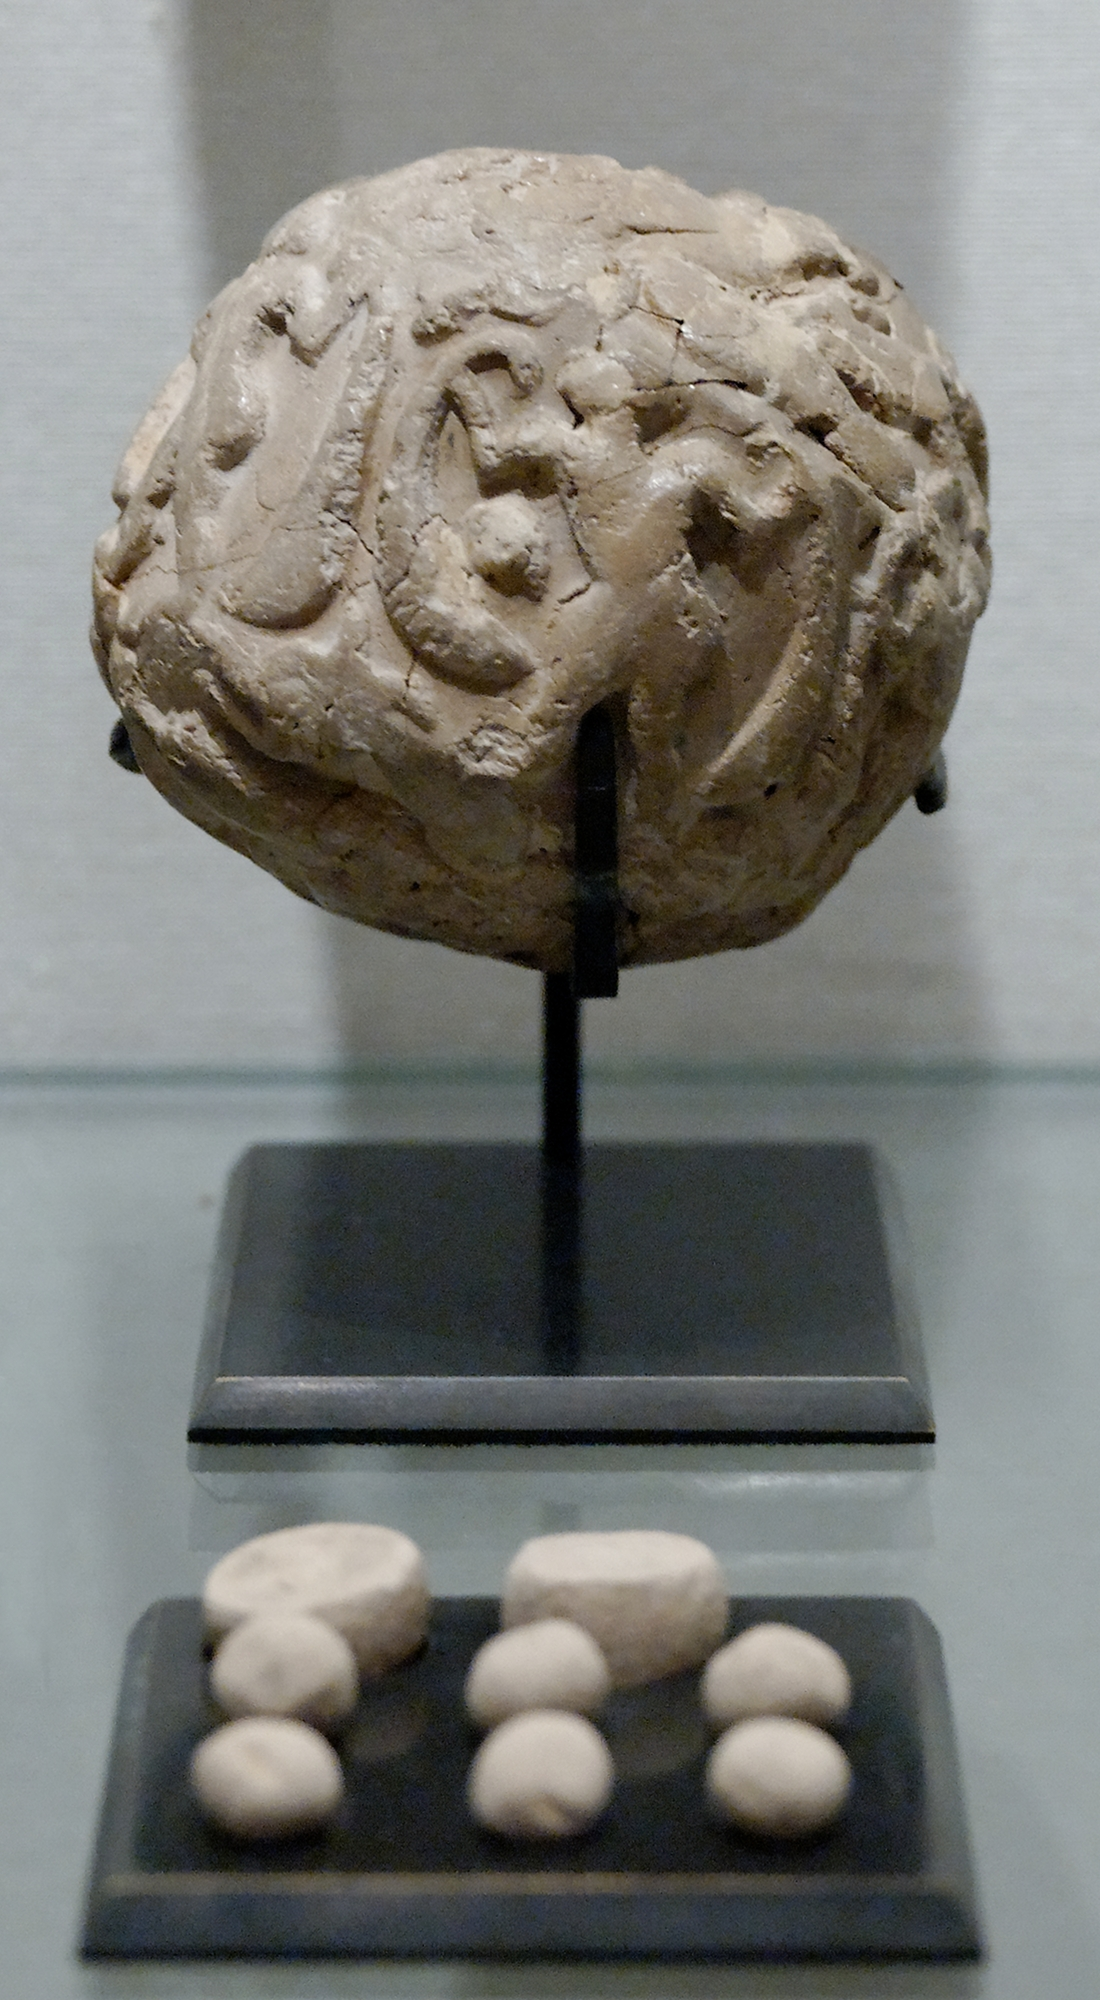
\includegraphics[scale=0.4]{img/clay-envelope.eps}
 \caption{卢浮宫陈列的乌鲁尔时期的计数陶罐和一组计数陶球。}
 \label{fig:clay-token}
%\end{figure}
\end{wrapfigure}

\underline{自}从人类进化开始,数的概念就伴随着我们。有人认为,数直接催生了人类的语言和文字。我们的祖先在长期的狩猎——采集活动中,逐渐掌握了数的概念。
最早可能是简单的数数,例如数清果实的数量。随着文明的发展,人们逐渐开始进行物品交易。随着交易物品数量增长,很快需要采用助记工具来处理更大的数。
考古发现在今天的伊朗一代,人们在公元前4000年开始使用陶制的小球来辅助计数。比如用两个刻有十字的小球代表两只羊,同时还有代表十只羊,二十只羊的不同小球。
为了防止忘记或者篡改数过的数目,人们还把这些小球放在陶罐中用泥土封存起来。图\ref{fig:clay-token}是乌鲁克(Uruk)时期的陶制计数罐和小球\cite{wiki-number}。
交易过程中,人们可以通过这些工具掌握货物的数量\cite{trip-to-number-kindom}。

\underline{然}而随着交易的增加和数目的增大,这样的陶罐和小球就不够方便了。大约公元前3500年,美索不达米亚的苏美尔人开始在泥板上刻化符号来纪录交易。将泥板烤硬后就可以方便的保存纪录。人们在这一时期用坚硬的笔在泥板上刻出不同的符号,同时表示交易的物品和数量。比如用一个象形符号表示五头牛,而用另一个象形符号表示十只羊。

\underline{数}的更大进步发生在公元前3100年,从出土的泥板中,我们发现苏美尔人开始将数字从它代表的物品中抽象出来。人们不再使用一个符号同时表示物品和数量,而是用一个符号表示交易的数量,接下来用另一个符号表示交易的物品。例如先用一个符号表示五,然后跟上一个牛的象形符号表示五头牛;而表示五只羊的时候,人们用同样的符号表示五,然后再跟上一个羊的符号。这些泥板上的符号逐渐演变成了古巴比伦的楔形文字。

%\begin{wrapfigure}{R}{0.5\textwidth}
\begin{figure}[htbp]
 \centering
 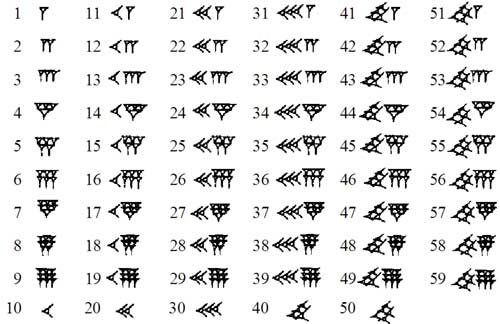
\includegraphics[scale=0.6]{img/Babylonian_numerals.eps}
 \caption{巴比伦楔形文字中的数字\cite{wiki-babylonian-num}。}
 \label{fig:babylonian-num}
\end{figure}
%\end{wrapfigure}

\underline{产}生抽象的数是智慧生命思维的结果。人们发现三个鸡蛋、三棵树、三个陶罐都可以用数字三来表示。这是一种强大的工具。从此,我们可以对抽象的数字进行操作,然后再把结果应用到各种具体事物上。例如我们可以把抽象的数字三加上一得到四,从而知道捡拾三个鸡蛋后再捡拾到一个鸡蛋会得到四个鸡蛋。同时我们也知道烧制三个陶罐后再烧制一个陶罐会得到四个陶罐。人们逐渐从解决单一问题发展到解决一类问题。

%\begin{wrapfigure}{R}{0.5\textwidth}
\begin{figure}[htbp]
 \centering
 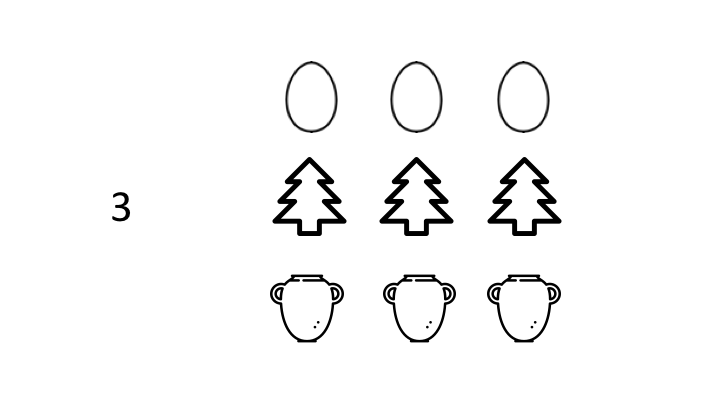
\includegraphics[scale=0.2]{img/abstract-num.eps}
 \caption{具体的三个事物和抽象的数字三。}
 \label{fig:abstract-num}
\end{figure}
%\end{wrapfigure}

\underline{生}产劳动中从数数开始,我们的老祖先逐渐发展出了操作抽象数字的方法,包括数字的加法、减法,更为强大的乘法,以及用于分配事物的除法。在丈量分割土地,计算谷物容量时,又逐渐将抽象的数和几何量联系起来。各个文明几乎分别独立的发现了数与形的内在规律。我们发现古埃及,古希腊,古中国都各自发现了毕达哥拉斯定理(勾股定理),古埃及人把它用于金字塔建造这样的伟大工程实践。从现代文明追根溯源,我们可以说自然数是数学和自然科学这条长河的源头。德国数学家克罗内克(Kronecker)说“上帝创造了自然数,其余都是人的工作。”\footnote{一说为整数,我们会在后继关于康托尔和无穷的章节再次提到克罗内克。}

\section{皮亚诺自然数公理}

%\begin{wrapfigure}{R}{0.4\textwidth}
\begin{figure}[htbp]
 \centering
 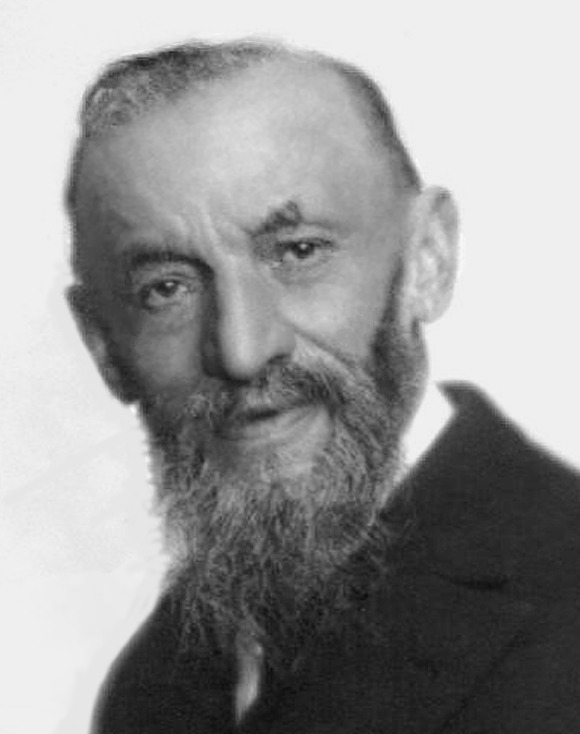
\includegraphics[scale=0.2]{img/Peano.eps}
 \caption{朱塞佩$\cdot$皮亚诺(Giuseppe Peano)1858 - 1932。}
 \label{fig:abstract-num}
\end{figure}
%\end{wrapfigure}

古希腊的欧几里得在他的伟大著作《几何原本》中开创了公理化的方法。他用五条公理和五条公设作为基石,精心构建一条一条定理的证明。每一个结论都仅仅使用公理和此前已经证明的定理。最终构建出了叹为观止的几何大厦。然而对于自然数,长期以来人们却没有建立起它的公理化形式系统。也许人们一直认为自然数的结论是直观和显而易见的。直到1889年,意大利数学家皮亚诺\footnote{皮亚诺不仅是数学家和逻辑学家,还是语言学家。他是数理逻辑和集合理论的先驱。他直接影响了罗素和怀特海的著作《数学原理》以及此后法国布尔巴基学派的纲领。他还创立了国际语(又称为“无屈折拉丁语”的人工语言)。}才为自然数建立起了严格的公理化系统。这就是著名的皮亚诺公里(Peano Axioms)。也许是上帝的巧合,欧几里得几何公理有五条,皮亚诺公理也有五条:


\begin{enumerate}
\item 0是自然数。用符号表示为$\exists 0 \in N$;
\item 每个自然数都有它的下一个自然数,称为它的后继。用符号表示为$\forall n \in N, \exists n' = succ(n) \in N$;
\end{enumerate}

似乎仅仅有这两条公理,我们已经能够定义出无穷无尽的自然数了,从0开始,下一个是1,下一个是2,接下来是3,……,接下来是某个$n$,下一个是$n+1$,……以至无穷。但是好挑刺的数学家给出了一个反例:考虑只有两个元素$\{0, 1\}$组成的数字系统,定义1的后继为0,0的后继为1。这样也满足上面的两条公理,却不是我们想像中的自然数

为此我们还需要第三条皮亚诺公理来排出这种情况。

\begin{enumerate}
  \setcounter{enumi}{2}
  \item 0不是任何自然数的后继。用符号表示为$\forall n \in N: n' \neq 0$;
\end{enumerate}

仅仅有这三条公理就够了么?我们还可以给出一个反例:考虑有限元素$\{0, 1, 2\}$组成的数字系统,定义0的后继是1,1的后继是2,2的后继还是2。这样也能满足上述三条公理。为此我们还需要第四条皮亚诺公理。

\begin{enumerate}
  \setcounter{enumi}{3}
  \item 不同的自然数有不同的后继数。或者说,如果两个自然数的后继数相同,那么这两个自然数相等。用符号表示为$\forall n, m \in N: n' = m' \Rightarrow n = m$;
\end{enumerate}

但是,仅仅用这四条公理仍然不够,因为可以存在这样的反例:考虑集合$\{0, 0.5, 1, 1.5, 2, 2.5, ...\}$,定义0的后继是1、1的后继是2……,0.5的后继是1.5、1.5的后继是2.5……但0.5不是任何元素的后继。为了排除这样的含有“不可达”元素的反例,还需要最后一条皮亚诺公理。

\begin{enumerate}
  \setcounter{enumi}{4}
  \item 如果自然数的某个子集包含0,并且其中每个元素都有后继元素。那么这个子集就是全体自然数。用符号表示为$\forall S \subset N: (0 \in S \land \forall n \in S \Rightarrow n' \in S) \Rightarrow S = N$.
\end{enumerate}

为什么公理5可以排出掉上述的反例呢?我们考虑集合$\{0, 0.5, 1, 1.5, 2, 2.5, ...\}$的一个子集$\{0, 1, 2, ...\}$。它包含0,并且每个元素都有后继元素,但是它不等于原集合。因为1.5、2.5……都不在这个子集中。所以它不满足第五条公理。公理五还有另外一个响亮的名字——归纳公里(Axiom of induction),它可以这样等价地描述:

\begin{enumerate}
  \setcounter{enumi}{4}
  \item 任意关于自然数的命题,如果证明了它对自然数0是对的,又假定它对自然数$n$为真时,可以证明它对$n'$也真,那么命题对所有自然数都真。(这条公理保证了数学归纳法的正确性)
\end{enumerate}

以上就是完整的五条皮亚诺公理,用它们可以构建出一阶算术系统,也称为皮亚诺算术系统\footnote{也有人从1开始,而不是0开始计算自然数。在皮亚诺当年的著作中,五条公理的顺序与此不同,其中第五条归纳公理被写在第三的位置上。}。

\section{自然数和计算机程序}
现代的计算机系统和在其上构建的程序已经非常的复杂和宏伟了。人们并非是先建立了计算机程序的公理系统,然后逐渐演绎出这些成果的。而是先取得了应用的巨大成功,然后才逐渐将计算机科学的基石数学化、形式化、严谨化的。这种有趣的现象在人类历史上已经不是第一次了。牛顿和莱布尼茨在17世纪发展了微积分,然后在几代数学家的手里应用到了各种领域,包括流体力学,天文学等等。但是直到19世纪才由柯西将微积分的理论严格化。

我们也模仿一下这样的过程,看看如何根据皮亚诺公理,用计算机程序定义自然数。在一个没有0、1、2、……这些我们熟悉的数字的程序系统中,我们可以这样定义自然数\footnote{本书使用一种理想的计算机语言,并在每一章节的最后给出真实计算机语言的参考代码。}:

\lstset{language=Haskell}
\begin{lstlisting}
data Nat = zero | succ Nat
\end{lstlisting}

%% \[
%% N \triangleq zero | succ(N)
%% \]

这一定义说:一个自然数或者为零,或者是另一自然数的后继。这里符号“|”表示互斥的关系。它自然蕴含了零不是任何自然数后继这一公理。在这一定义下,我们可以进一步定义出自然数的加法。

\begin{lstlisting}
a + zero = a
a + (succ b) = succ (a + b)
\end{lstlisting}

加法定义包含两部分。首先任何自然数和零相加等于它本身;并且某个自然数和另一个数的后继相加,等于这两个数相加的后继。写成数学符号为:

\be
\begin{array}{l}
a + 0 = a \\
a + b' = (a + b)'
\end{array}
\ee

我们来验证一下2+3。自然数2为succ(succ zero),而3为succ(succ(succ zero))。根据加法的定义2+3为:

\begin{lstlisting}
  succ(succ zero) + succ(succ(succ zero))
= succ(succ(succ zero) + succ(succ zero))
= succ(succ(succ(succ zero) + succ zero))
= succ(succ(succ(succ(succ zero) + zero)))
= succ(succ(succ(succ(succ zero))))
\end{lstlisting}

最终结果的确是零的五重后继,也就是5。从零开始一次一次的重复使用后继函数的记法很麻烦。如果要表示100,这种记法要写很多行并且容易出错。为此,我们用下面的简单记法表示自然数$n$:

\be
n = foldn(0, succ, n)
\ee

它表示从零开始,不断叠加使用succ函数$n$次。$foldn$函数可以具体实现如下:

\be
\begin{array}{l}
foldn(z, f, 0) = z \\
foldn(z, f, n') = f(foldn(z, f, n))
\end{array}
\label{eq:foldn}
\ee

$foldn$定义了在自然数上的一种操作,只要令$z$为$zero$,令$f$为$succ$就可以实现叠加后继若干次,从而获得某个特定的自然数。我们可以用前几个自然数验证一下:

\begin{lstlisting}
foldn(zero, succ, 0) = zero
foldn(zero, succ, 1) = succ(foldn(zero, succ, 0)) = succ zero
foldn(zero, succ, 2) = succ(foldn(zero, succ, 1)) = succ(succ zero)
...
\end{lstlisting}

定义好加法之后,我们再来定义自然数的乘法:

\begin{lstlisting}
a . zero = zero
a . (succ b) = a . b + a
\end{lstlisting}

这里我们使用了刚才定义好的加法。这一定义写成数学符号为:

\be
\begin{array}{l}
a \cdot 0 = 0 \\
a \cdot b' = a \cdot b + a
\end{array}
\ee

\begin{wrapfigure}{R}{0.4\textwidth}
\centering
\begin{tikzpicture}[scale=0.8]
\filldraw[pattern=north west lines] (0, 0) rectangle (2, 1)
    (2, 0) rectangle (3, 1);
\draw (3, 0) rectangle (4.5, 1);
\draw (0, -1) rectangle (2, -2);
\filldraw[pattern=north west lines] (2, -1) rectangle (3, -2)
    (3, -1) rectangle (4.5, -2);
\end{tikzpicture}
\caption{加法结合律的几何证明。上下面积相等}
\end{wrapfigure}

与通常的观念不同,加法和乘法的交换律、结合律既不是公理,也不是公设。它们都是可以用皮亚诺公理和加法的定义严格证明的定理。我们来看看证明加法结合律的例子。加法结合律是说$(a + b) + c= a + (b + c)$。我们先证明当$c=0$时它是对的。根据加法定义的第一条规则:

\[
\begin{array}{rl}
(a + b) + 0 & = a + b \\
            & = a + (b + 0)
\end{array}
\]

然后是递推步骤,假设$(a + b) + c = a + (b + c)$成立,我们要推出$(a + b) + c' = a + (b + c')$。

\[
\begin{array}{rlr}
(a + b) + c' & = (a + b + c)' & \text{加法定义的第二条规则} \\
             & = (a + (b + c))' & \text{递推假设} \\
             & = a + (b + c)' & \text{加法定义的第二条规则} \\
             & = a + (b + c') & \text{加法定义的第二条规则}
\end{array}
\]

这样我们就证明了加法的结合律。但是加法交换律的证明却并不简单,附录一给出了完整的证明。

%\begin{wrapfigure}{R}{0.4\textwidth}
\begin{figure}[htbp]
\centering
\begin{tikzpicture}[scale=0.8]
\draw (0, 0) rectangle (2, 1)
    (2, 0) rectangle (3, 1);
\draw (0, -1) rectangle (1, -2)
    (1, -1) rectangle (3, -2);
\end{tikzpicture}
\caption{加法交换律的几何证明。将上方的图形倒过来看,或者在镜中看}
\end{figure}
%\end{wrapfigure}

\begin{Exercise}
\begin{enumerate}
\item 定义0的后继为1,证明对于任何自然数都有$a \cdot 1 = a$
\item 证明乘法结合律和交换律
\item 证明乘法分配律
\end{enumerate}
\end{Exercise}

\section{自然数的结构}
有了加法和乘法,我们就可以定义更复杂的计算。第一个例子是从零开始的累加:$0 + 1 + 2 + ... $

\be
\begin{array}{l}
sum(0) = 0 \\
sum(n + 1) = (n + 1) + sum(n)
\end{array}
\ee

第二个例子是阶乘$n!$。

\be
\begin{array}{l}
fact(0) = 1 \\
fact(n + 1) = (n + 1) \cdot fact(n)
\end{array}
\ee

比较这两个例子,我们发现它们非常相似。尽管人工智能日新月异地发展,智慧生命和智能机器的一大区别就是能否“跳出系统”,到更高的层次进行抽象。这是我们人类心智中最强大、神秘、复杂、难以捉摸的一部分\cite{GEB}。

我们发现累加和阶乘都有一个针对自然数零起始值,累加始自零,阶乘始自一。针对递归情况,它们都将某一操作应用到一个自然数和它的后继上。累加是$n' + sum(n)$,阶乘是$n' \cdot fact(n)$。如果我们把针对零的起始值抽象为$c$,把递归中的操作抽象为$h$,就可以用一个统一的形式概括累加和阶乘。

\be
\begin{array}{l}
f(0) = c \\
f(n + 1) = h(f(n))
\end{array}
\ee

这是一个在自然数上的递归结构。我们观察一下它在前几个自然数上的表现。

\begin{tabular}{l|l}
$n$ & $f(n)$ \\
\hline
0 & $c$ \\
1 & $f(1) = h(f(0)) = h(c)$ \\
2 & $f(2) = h(f(1)) = h(h(c))$ \\
3 & $f(3) = h(f(2)) = h(h(h(c)))$ \\
... & ... \\
$n$ & $f(n) = h^n(c)$
\end{tabular}

其中,$h^n(c)$表示我们叠加在$c$上重复进行$n$次$h$操作。它是\underline{原始递归}形式的一种(\cite{Bird97},第5页)。更进一步,如果观察此前我们在(\ref{eq:foldn})定义的函数$foldn$,就会发现它们之间的关系:

\be
f = foldn(c, h)
\ee

细心的读者会观察到,我们最初定义的$foldn$带有三个参数,为什么这里只有两个了呢?实际上我们可以写成$f(n) = foldn(c, h, n)$。当我们仅传递给三元函数$foldn$前两个参数,它实际上就成为了接受一个自然数为参数的一元函数了。我们可以这样看待它:$foldn(c, h)(n)$。

我们称$foldn$为自然数上的$fold$操作。令$c$为$zero$,$h$为$succ$,我们就得到了自然数。如同上面的表格,我们可以得到一个序列:

\[
zero, succ(zero), succ(succ(zero)), ... succ^n(zero), ...
\]

如果$c$不是$zero$,$h$不是$succ$,则$foldn(c, h)$就描述了和自然数同构的某种事物。我们来看几个例子:

\[
(+ m) = foldn(m, succ)
\]

这个例子描述了将自然数$n$增加$m$的操作,将它依次作用到自然数上可以产生和自然数同构的序列$m, m + 1, m + 2, ..., n + m, ...$

\[
(\cdot m) = foldn(0, (+ m))
\]

这个例子描述了将自然数$n$乘以$m$的操作,将它依次作用到自然数上可以产生和自然数同构的序列$0, m, 2m, 3m, ..., nm, ...$

\[
m^{()} = foldn(1, (\cdot m))
\]

这个例子描述了对自然数$n$取$m$次幂的操作,将它依次作用到自然数上可以产生和自然数同构的序列$1, m, m^2, m^3, ..., m^n, ...$

那么,我们思考出的这个抽象工具$foldn$能否描述累加和阶乘呢?我们观察下面的这个表格:

\begin{tabular}{r|l|l|l|l|l|l}
$n$ & 0 & 1 & 2 & 3 & ... & $n'$ \\
\hline
$sum(n)$ & 0 & 1 + 0 = 1 & 2 + 1 = 3 & 3 + 3 = 6 & ... & $n' + sum(n)$ \\
\hline
$n!$ & 1 & 1 $\times$ 1 = 1 & 2 $\times$ 1 = 2 & 3 $\times$ 2 = 6 & ... & $n' \cdot (n!)$
\end{tabular}

这里的关键问题是$h$必须是个二元操作,它能够对$n'$和$f(n)$进行运算。为此,我们将$c$也定义为一个二元数$(a, b)$\footnote{在计算机程序中,也称为二元组(tuple),或者对(pair)。}。然后针对二元数$(a, b)$定义某种类似“succ”的操作。最终为了获取结果,我们还需要要定义从二元数中抽取$a$和$b$的函数:

\be
\begin{array}{l}
1st (a, b) = a \\
2nd (a, b) = b
\end{array}
\ee

这样我们就可以定义累加和阶乘了。首先是累加的定义:

\[
\begin{array}{lr}
c = (0, 0) & \text{二元数的起始值} \\
h (m, n) = (m', m' + n) & \text{第一个数取后继,第二个数加第一个数的后继} \\
sum = 2nd \cdot foldn(c, h) \\
\end{array}
\]

我们看看,从起始值$(0, 0)$开始,会怎样一步一步递推出累加的结果。

\begin{tabular}{r|l|l}
$(a, b)$ & $(a', b') = h (a, b)$ & $b'$\\
\hline
(0, 0) & (0 + 1 = 1, 1 + 0 = 1) = (1, 1) & 1 \\
(1, 1) & (1 + 1 = 2, 2 + 1 = 3) = (2, 3) & 3 \\
(2, 3) & (2 + 1 = 3, 3 + 3 = 6) = (3, 6) & 6 \\
... & ... & ... \\
$(m, sum(m))$ & $(m + 1, m + 1 + sum(m))$ & $sum(m + 1)$
\end{tabular}

类似地,我们用$foldn$定义出阶乘。

\[
\begin{array}{lr}
c = (0, 1) & \text{阶乘的起始值} \\
h (m, n) = (m', m'n) & \text{阶乘的递推} \\
fact = 2nd \cdot foldn(c, h) \\
\end{array}
\]

在累加和阶乘的定义中,我们使用了符号“$\cdot$”点来连接两个函数$2nd$和$foldn(c, h)$。我们称之为函数组合,$f\cdot g$表示先将函数$g$应用到变量上,然后再将函数$f$应用到结果上。即$(f\cdot g)(x) = f(g(x))$。

\begin{wrapfigure}{R}{0.4\textwidth}
%\begin{figure}[htbp]
 \centering
 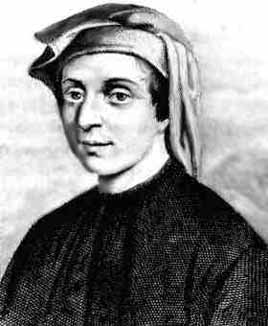
\includegraphics[scale=0.4]{img/Fibonacci.eps}
 \caption{比萨的列奥纳多,又称斐波那契(Leonardo Pisano, Fibonacci),1175年-1250年}
 \label{fig:abstract-num}
%\end{figure}
\end{wrapfigure}

为了展示这一抽象工具的强大,我们再来看一个例子:斐波那契数列。这一数列是用中世纪数学家比萨的列奥纳多命名的。斐波那契来自拉丁文filius Bonacci意思是波那契之子。斐波那契的父亲当时是商人,在北非以及地中海一带经商,斐波那契逐渐向当地阿拉伯人学习了印度——阿拉伯的数字系统并通过他的著作《算盘书》(Liber Abaci)将其介绍到欧洲。中世纪的欧洲一直使用罗马数字系统,我们今天在一些钟表盘上仍然可以看到罗马数字。例如2018年的罗马数字表示为MMXVIII,其中一个M代表1000,两个M代表2000,X代表10,V表示5,三个I表示3。把这些加起来得到2018。斐波那契引入欧洲的是我们今天仍然使用的位值制十进制系统。它使用了印度数学发明的零,不同的数字在不同的位置上含义不同。这一先进的数字系统极大地方便了计算,广泛应用在记账、利息、汇率等方面。《算盘书》更是对欧洲的数学复兴产生了深远的影响。

斐波那契数列来自《算盘书》中的一个问题:兔子在出生两个月后,就有繁殖能力,一对兔子每个月能生出一对小兔子来。如果所有兔都不死,那么一年以后可以繁殖多少对兔子?开始时有一对兔子。第一个月小兔尚未具备繁殖能力,所以仍然只有一对兔子。第二个月它们生下一对小兔,共有两对。第三个月大兔子又生下一对小兔,而上月生的小兔还在成长,总共有2+1=3对。第四个月有两对大兔子产下两对小兔,加上原有的三对兔子,总共有3+2=5对。按照这样,我们可以得到一个序列

1, 1, 2, 3, 5, 8, 13, 21, 34, 55, 89, 144, ...

这个数列很有规律,从第三项后,任何一项都等于前两项的和。我们可以这样思考它的原理,如果前一个月有$m$对兔子,这个月有$n$对兔子,那么增加的一定都是新产下的小兔,共有$n-m$对,而剩下的都是成年兔子,共$m$对。到下个月时,这$n-m$对小兔刚刚成熟,而$m$对成兔又产下了$m$对小兔。所以下个月的兔子总数等于小兔加上成兔为:$(n - m) + m + m = n + m$对。根据这一推理,我们可以给出斐波那契数列的递归定义:

\be
\begin{array}{l}
F_0 = 0 \\
F_1 = 1 \\
F_{n+2} = F_n + F_{n+1}
\end{array}
\ee

习惯上通常将斐波那契数列的起始值定义为0和1\footnote{如果起始值是1和3,我们就得到了卢卡斯数列1, 3, 4, 7, 11, 18, ...}。注意到斐波那契数列的起始值是一对自然数,并且递推关系也是一对值。我们可以利用抽象工具$foldn$给出下面的定义\footnote{在介绍康托尔的无穷概念时,我们会给出另一个斐波那契数列的定义。}:

\be
\begin{array}{l}
F = 1st \cdot foldn((0, 1), h) \\
h (m, n) = (n, m + n)
\end{array}
\ee

也许读者会好奇,真实的计算机程序能实现这样的定义么?这是不是太理想化了?下面方框是一段的Haskell语言的程序代码\footnote{2010年后,Haskell中不再允许使用n+k形式的模式匹配,可以修改为:\newline\texttt{foldn z f n = f (foldn z f (n - 1))}},执行\texttt{fib 10}会输出斐波那契数55\footnote{一行代码输出前100个斐波那契数的例子:\newline\texttt{take 100 \$ map fst \$ iterate ($\lambda$(m, n)->(n, m + n)) (0, 1)}}。

\lstset{frame=single}
\begin{lstlisting}
foldn z _ 0 = z
foldn z f (n + 1) = f (foldn z f n)

fib = fst . foldn (0, 1) h where
  h (m, n) = (n, m + n)
\end{lstlisting}

\begin{Exercise}
\begin{enumerate}
\item 使用$foldn$定义$()^m$,计算给定自然数的$m$次幂。
\item 使用$foldn$定义平方。
\item 使用$foldn$定义奇数的平方和。它会产生怎样的序列?
\end{enumerate}
\end{Exercise}

%\begin{wrapfigure}{R}{0.3\textwidth}
\begin{figure}[htbp]
 \centering
 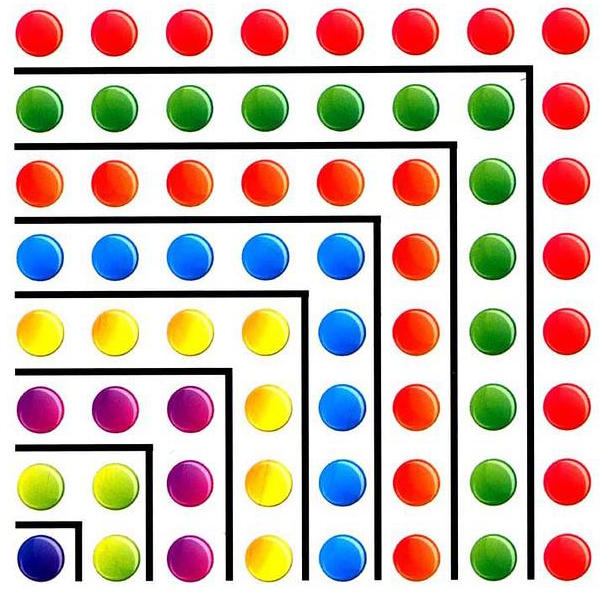
\includegraphics[scale=0.2]{img/PWW.eps}
 \caption{《无需语言的证明》封面局部}
 \label{fig:PWW}
\end{figure}
%\end{wrapfigure}

\section{自然数的同构}

自然数不仅可以和自己的子集同构,例如奇偶数、平方数、斐波那契数,还可以和其他事物同构。其中一个例子是计算机程序中的数据结构。下面是列表的定义

\section{形式与结构}

TODO: 换为《雅典学院》
\begin{wrapfigure}{R}{0.3\textwidth}
%\begin{figure}[htbp]
 \centering
 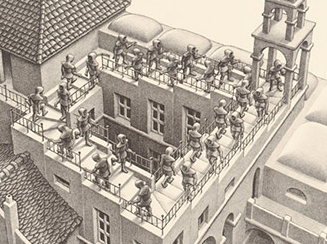
\includegraphics[scale=0.4]{img/Escher-AnD.eps}
 \caption{埃舍尔作品《上升与下降》局部}
 \label{fig:Escher-AnD}
%\end{figure}
\end{wrapfigure}

你也许注意到了本章第一节中,每个自然段的开头的第一个汉字连起来是“自然数产生”,我希望用这种形式表达同构的美。

\ifx\wholebook\relax \else
\begin{thebibliography}{99}

\bibitem{wiki-number}
Wikipedia. ``古代计数系统的历史''. \url{https://en.wikipedia.org/wiki/History_of_ancient_numeral_systems}

\bibitem{trip-to-number-kindom}
[美]卡尔文$\cdot$C$\cdot$克劳森. ``数学旅行家:漫游数王国''. 袁向东、袁钧译,上海教育出版社。ISBN:

\bibitem{wiki-babylonian-num}
Wikipedia. ``古巴比伦数字''. \url{https://en.wikipedia.org/wiki/Babylonian_numerals}

\bibitem{GEB}
[美]候世达 ``哥德尔、埃舍尔、巴赫——集异壁之大成''. 商务印书馆 1996. ISBN: 978-7-100-01323-9

\bibitem{Bird97}
Richard Bird, Oege de Moor. ``Algebra of Programming''. Univerisity of Oxford, Prentice Hall Europe. 1997. ISBN: 0-13-507245-X.

\end{thebibliography}

\expandafter\enddocument
%\end{document}

\fi
